\section{Implementation}\label{sec:implem}

YETI is an application coded in Java, allowing to test programs at random in a fully automated manner.
It is designed to support various programming languages -- for example, functional, procedural and object-oriented languages can easily be supported.
 It contains three parts: the core infrastructure, the strategy, and the language-specific bindings. 
YETI is a lightweight platform with around 5000 lines of code for the core, strategies and the Java binding.
 As explained in Section~\ref{sec:model}, the core infrastructure provides extendibility trough specialization. 
 To create specific strategies or language bindings, one subclasses abstract Java classes.

\subsection{Using YETI}
YETI is a tool that can be launched on the command-line. A typical call of YETI is:
{\small
\begin{verbatim}
java yeti.Yeti -Java -yetiPath=. -time=10mn -randomPlus
-testModules=java.lang.String:java.lang.StringBuilder 
\end{verbatim}
}

The options used on this command-line have the following meaning: \texttt{-Java} 
indicates that the tested program is in Java, \texttt{-yetiPath=.} indicate that 
classes in the current directory (and its subdirectories) will be preloaded, 
\texttt{-time=10mn} indicates that the testing session will last 10 minutes, 
\texttt{-randomPlus} indicates that the strategy random+ will be used, and 
\texttt{-testModules=java.lang.String:...} indicates that 
both \texttt{String} and \texttt{StringBuilder} will both be tested.

While testing, traces of faults found are output to the terminal. For example:

{\small
\begin{verbatim}
Exception 5
java.lang.NullPointerException
        at java.lang.String.replace(String.java:2207)
\end{verbatim}
}

At the end of the testing sessions, YETI outputs generated test cases reproducing 
the faults found during the testing session as well: 

{\small
\begin{verbatim}
...
public static void test_5() throws Exception {
double v0=0.0d; // time:1254919729044
java.lang.String v1=java.lang.String.valueOf(v0); 
                                   // time:1254919729044
java.lang.String v25=new java.lang.String(); 
                                   // time:1254919729106
java.lang.String v26=v25.replace(null,v1); 
                                   // time:1254919729106
/**BUG FOUND: RUNTIME EXCEPTION**/ // time:1254919729114
/**YETI EXCEPTION - START 
java.lang.NullPointerException
        at java.lang.String.replace(String.java:2207)
YETI EXCEPTION - END**/ 
/** original locs: 59 minimal locs: 4**/
}
...
/** Non-Unique bugs: 223, Unique Bugs: 104, 
Logs size (locs): 2172**/
/** Testing Session finished, number of tests:1178, 
time: 1007ms, number of failures: 223**/
/** Processing time: 3119ms **/
/** Testing finished **/
\end{verbatim}
}

Note that it is also possible to avoid the overhead of keeping the 
traces in the system (and calculating the minimal test cases) by specifying 
\texttt{-nologs} to throw away all logs except exception traces, or 
\texttt{-rawlogs} to output the logs to the terminal.

\subsection{Graphical User Interface (GUI)}
By specifying the \texttt{-gui} option, YETI shows a graphical user interface
that allows test engineers to interact directly with the system while the testing 
session proceeds. 

\begin{figure}[h!]
\begin{center}
\begin{sideways}
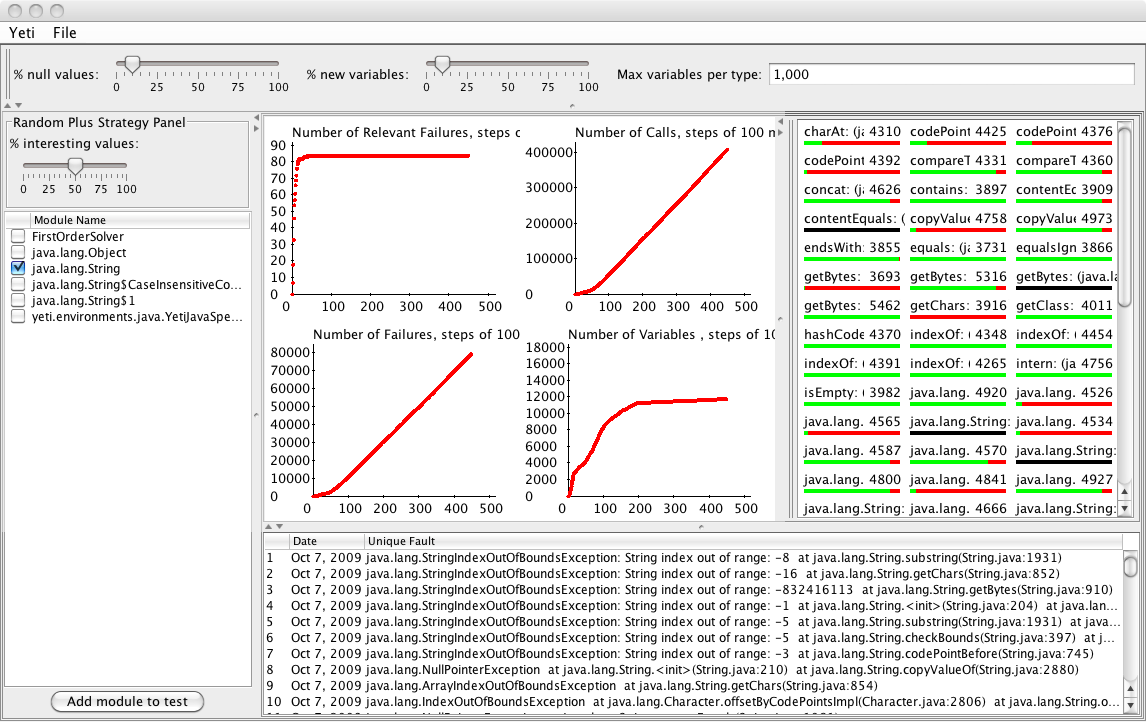
\includegraphics[width=16cm]{images/YetiComplete.png}
\end{sideways}
\end{center}
\caption{YETI graphical user interface.}\label{fig:gui}
\end{figure}

Figure~\ref{fig:gui} shows YETI's graphical user interface when using 
the random+ strategy. At the top of the interface, two sliders correspond to 
the percentage of null values and the percentage of new variables to use when testing.
In short, each time a test is made, each parameter of the routine to test can either 
be void, newly generated or a new variable. These sliders indicate which probability 
to use. In the top part there is also a text field to limit the number of instances per 
type in the system (which is necessary for long-running sessions).

The left panel contains a panel specific to the current strategy (in the example, the 
considers using ``interesting'' values when possible) and a list of modules loaded in 
the system. The modules being tested are ticked, while others can be used as helpers to 
create variables to use on-demand making a routine calls. A button is available to add modules 
at runtime for programming languages that support it. This last part is useful in cases 
where a module is missing for being able to test routine. 

In the central panel, four graphs describe the evolution of the system: the top-left one shows 
the evolution of the number of unique failures found -- all failures without redundancy --, the 
bottom-left indicates the raw number of failures over time, the bottom-right indicates the current 
number of instances in the system, the top-right panel indicates the total number of calls effected by YETI.

The panel on the right shows all methods tested in the system and presents results in the form 
of a colored gauge where black indicates that the routine was not tested, green is the proportion
of routines tested successfully, yellow represents routine calls that cannot be interpreted
-- for example,	 YETI had to stop a thread --, and red indicates failures.

The bottom panel reports unique failures as they are found: each line is a unique failure.

In order for the graphical interface not to slow down the testing process, we use two threads.
The first one samples data for building graphs every .1 seconds, the second one updates the graphical user interfaces and waits .1 second between two updates. A special care has also been taken for not showing all samples in the graphs when not needed: we only show one point per pixel on the x-axis. In ten minutes testing sessions  of \texttt{java.lang.String} on a dual core MacBook Pro, the slowdown incurred by the GUI was $4.4\%$. 

\subsection{Core Architecture}
The core architecture of YETI is consistent with the model described in Section~\ref{sec:model}.
YETI uses the core notions of types, routine, modules and variables by defining respectively Java classes 
\texttt{YetiType}, \texttt{YetiRoutine}, \texttt{YetiModule}, and \texttt{YetiVariable}.
YETI also maintains the types so that the constraints on Figure~\ref{fig:subtype} are naturally respected.

The primitives and instructions are implemented either in language-specific classes or in 
strategy-specific classes through abstract classes that must be implemented.

\subsection{Java Binding}
The Java binding redefines classes from the base framework to let YETI test Java programs.
It is currently the reference implementation for making new bindings for YETI.
The Java binding uses class loaders to find definitions of classes it tests. It uses 
reflection to make calls. Tests are run in a separate thread so that infinite loops can be 
stopped. The next paragraphs explain each of these points in more detail.

\paragraph{Custom class loader.}
The Java binding defines a custom class loader mainly to perform two tasks: prefetching classes in 
the \texttt{-yetiPath} option and create types and modules from classes loaded in YETI.

Prefetching classes is effected as soon as YETI starts, it consists in loading all classes in a given 
path. Each of these classes then defines both a module and a type. By default, None of the classes in the transitive closure of classes defines either a module or a type. This is mainly due to performance optimizations as this would automatically result in loading at least 30 classes in the system, 
some of which have a very negative impact on performances of the system (for example 
\texttt{java.lang.StringBuffer}). Instead, test engineers might decide to load such classes 
-- or other helper classes -- through the graphical user interface.

Subsequently to loading, each method of each loaded class is added to its module, while any method (including 
constructors) returning an object of a given type is added as a ``constructor'' for that type.

\paragraph{Reflection.} The Java binding subclasses \texttt{YetiRoutine} with two classes: \texttt{YetiJava- Constructor} and \texttt{YetiJavaMethod}. Each of these classes uses reflection to make 
the calls.

\paragraph{Threads.} The Java binding uses two threads: a worker thread to perform tests and a second to control -- and possibly stop --�the first one. Associated to the thread group of the worker thread,
we use the Java security model and do not grant any permission. That way, the code cannot create files, 
open sockets, or in general do any potentially dangerous operation. The only operation not ruled out is 
exiting the program. Note also that we forbid the system to test \texttt{wait}, \texttt{notify}, and \texttt{notifyAll}.


\subsection{Strategies}
By default YETI contains four main strategies:
\begin{description}
\item[Pure random] is a strategy that generates calls and selects values at random. Two main probabilities can be used: the percentage of null values, and the percentage of newly created objects to use when testing.
\item[Random+] adds the utilisation of ``interesting'' values. For the Java binding such values for integers contain \texttt{MAX\_INT}, \texttt{MIN\_INT}, all values between $-10$ and $10$ etc. It also defines the probability to use such interesting values.
\item[Random Decreasing] is a random+ strategy where all three probabilities start at $100\%$ and then linearly decrease until they are at $0$ at the end of the session.
\item[Random Periodic] is a random+ strategy where all three probabilities periodically decrease and increase over the testing session.
\end{description}

While the first two strategies were described previously in literature~\cite{CMOP:08:FFMTRTUR}, the last two are new as nobody thought of modifying the probabilities over time before.
